% !TEX program = xelatex
\documentclass{matthijs}
\graphicspath{{../assets/}{./docs/assets/}{./docs/technical-design/}}

% BEGIN preamble.tex

% Style for first and last page
\usepackage{wallpaper}
\usepackage{color}
\definecolor{arobsblue}{HTML}{0e335c}

% Versioning plugin that retrieves data from the git repo dir
% Needs the "gitInfoHead" file to be generated, make sure
% that the shim script or the git hook is enabled
\usepackage[maxdepth=2]{gitinfo2}

% Use biblatex with biber backend for bibliography
\usepackage{csquotes}
\usepackage[style=ieee]{biblatex}
\renewcommand*{\mkbibacro}[1]{#1}
\setcounter{biburllcpenalty}{7000}
\setcounter{biburlucpenalty}{8000}

% This lets the text look really juicy
\usepackage{microtype}
\usepackage{extdash}

% A column for right-aligned autowrap text
\newcolumntype{R}{>{\arraybackslash}m{10cm}}

% PDF-A
\usepackage{colorprofiles}
\usepackage[a-3b]{pdfx}
\hypersetup{
	bookmarks=true,
	unicode=false,
	pdftoolbar=true,
	pdfmenubar=true,
	colorlinks=true,
	linkcolor=black,
	citecolor=black,
	filecolor=black,
	urlcolor=black
}
%\hypersetup{
%	colorlinks=true,
%	linkcolor=gray,
%	urlcolor=gray,
%	citecolor=gray
%}

% END preamble.tex


\usepackage{titlepage}
\usepackage[title,titletoc]{appendix}

% Load bibliography file
\addbibresource{td.bib}

% Use tikz for drawings
\usepackage{tikz}
\usepackage{tikzscale}
\usepackage{tikz-uml}
\usetikzlibrary{positioning, arrows.meta}

\begin{document}

	% Set language to English
	\taal{en}

	\maketitlepage{Technical Design}{0.1}
	\pagenumbering{arabic}
	\thispagestyle{empty}

	\begin{inhoudspagina}

		\clearpage

		%\begin{table}[!ht]
			\begin{tabular*}{\textwidth}{l @{\extracolsep{\fill}} R}
				\toprule

				\textbf{Abbreviation} & \textbf{Definition} \\
				\midrule

				ADAS & Advanced Driver-Assistance System \tabularnewline
				ASIC & A non-reconfigurable digital circuit \tabularnewline
				AXIS & AXI Stream; a bus protocol for data streaming interfaces \tabularnewline
				DMA & Direct Memory Access; a way of reading from / writing to memory without utilizing a processor \tabularnewline
				FPGA & Field Programmable Gate Array; a customizable logic circuit \tabularnewline
				Hard-core processor & A dedicated processor as an ASIC \tabularnewline
				HLS & High Level Synthesis; a technique for synthesizing high level computer code to RTL \tabularnewline
				IPI & Vivado IP Integrator; a tool for integrating IP Cores into block designs \tabularnewline
				IP Core & A pre-made digital logic design \tabularnewline
				MPSoC & Multi-Processor SoC; a SoC with multiple physical processing cores; just a marketing term someone at Xilinx made up \tabularnewline
				PL & Programmable Logic; digital logic that can be reconfigured \tabularnewline
				PS & Processing System; everything related to hard- or softcore processors on the device \tabularnewline
				RTL & Register Transfer Level code; a way of describing the behavior of digital logic \tabularnewline
				SoC & System on Chip; a combination of PL and a hard-core processor \tabularnewline
				Soft-core processor & A processor which is implemented in programmable logic \tabularnewline
				VDMA & Video DMA; A DMA controller specially constructed to read/write video data \tabularnewline
				VPU & Vision Processing Unit; refer to chapter 2 of the Functional Design \tabularnewline

				\bottomrule
			\end{tabular*}
			%\label{tabel:Abbreviations}
		%\end{table}

		\vspace{3ex}

		\textbf{Note:} the abbrevation \textit{DRAM} is ambiguous and is often mixed up in FPGA literature.
		In some situations it means \textit{Distributed RAM} (the memory that can be instantiated in SLICEM LUTs~\cite{xilinxug474}) and in other situations it means \textit{Dynamic RAM} (the external memory that is implemented on our FPGA board).
		To avoid confusion, I will be using the abbrevation \textit{SDRAM} to reference the Dynamic RAM variant.

	\end{inhoudspagina}

	\pagenumbering{arabic}
	\tolerance=1
	\emergencystretch=\maxdimen
	\hyphenpenalty=10000
	\hbadness=10000

	\begin{hoofdstuk}{Preface}

		This project is centered around the realization of an ADAS subsystem which can detect the position of a vehicle within a lane.
		A camera is positioned on the dashboard facing the road in front of the vehicle.
		The video feed from this camera is analyzed in real-time by a computer vision system called the Vision Processing Unit.
		This system is implemented on a Field Programmable Gate Array to achieve low-latency detection.
		The output data, existing of information about the lane the car currently occupies, is passed on to the Lane Departure Warning System so that the car can make decisions with it.

		\bigskip

		This document pertains to the technical side of the system.
		The main goal of this document is to give insight on the inner workings of the system so that the knowledge is preserved and modifications to the system can be easily made in the future.
		Design choices and the overcoming of bottlenecks are mentioned to give advice for future projects.
		Another goal is to describe how the system is integrated in a vehicle so that technicians can troubleshoot issues with it.
		The target audience for this document is whom want to get hands-on with the system and its internals.

		\bigskip

		A global system overview is given in the first paragraph to provide context to the reader.
		In the following paragraphs, the layers of the system are described starting with the hardware layer and ending with the software layer.
		The hardware paragraph is about the physical hardware components which are used in the project.
		The programmable logic layer is about the register transfer level code and how it is synthesized on the FPGA.
		The processing system layer is about the program that runs on the processor.
		The software layer is about the troubleshooting software that runs on an external system and can be used by mechanics to see the internals of the processing unit.

		\bigskip

		In this document I will name binary quantities according to the binary multiples convention as described in ISO/IEC 60027-2:2019.
		E.g. one kilobit (Kb) is 1000 bits and one kibibit (Kib) is 1024 bits.

	\end{hoofdstuk}

	\begin{hoofdstuk}{System Overview}

		The goal of this paragraph is to describe the problem that the product will solve in different layers of complexity.
		Each layer will dissect the problem into more complexity than the previous.
		This approach gives context to readers who might not be familiar with the fine technical concepts and who wish to grasp the knowledge at a higher level.

		\begin{paragraaf}{Problem Domain}

			Although the system is not directly controlled by a user, many external forces influence the working of the system.
			We have to take them into account when developing the system because they may affect which choices we will make in the development process and how we integrate the system in a vehicle.

			\begin{figuur}{Operational Problem Domain}
				\singlespacing
				\includegraphics[width=\textwidth]{problem-domain}
				\onehalfspacing
			\end{figuur}

		\end{paragraaf}

		\begin{paragraaf}{Information Context}

		\end{paragraaf}

		\begin{paragraaf}{Component Definition}

			In order to describe which components make up the total system, I have modeled two SysML block diagrams; a Block Definition Diagram (BDD) and an Internal Block Diagram (IBD).
			The BDD shows the components that the system consists of and the Internal Block Diagram shows the relations and interfaces between these components.
			The BDD can be thought of as a black box view that does not represent the inner workings of the system but rather the specifications of it, while the IBD shows exactly how the system is internally composed.

			\begin{figuur}{The System as a SysML Block Definition Diagram}
				\singlespacing
				%\includegraphics[width=\textwidth]{block-definition-diagram}
				\onehalfspacing
			\end{figuur}

		\end{paragraaf}

		\
		\textbf{[todo:]}

	\end{hoofdstuk}

	\begin{hoofdstuk}{Integrated Block Design}

		The block design for the system has been created using the Vivado IP Integrator (IPI) because it is the recommended tool to integrate Xilinx IP like the Zynq Processing System in a digital design~\cite{xilinxug994}.
		The design consists of three important components which are connected by diverse utility components.
		These important components are the Zynq Processing System which connects to the hard-core ARMv9 processors, the AXI DMA interface which exchanges memory between PS/PL, and the VPU Image Processing IP Core which is generated by our High Level Synthesis routine.
		The utility components that 'glue' the system in place consist of Xilinx IP Cores like AXI Interconects that act like buses, AXI Stream Data Width converters that add/remove padding from the video streams and finally the Processor System Reset which manages the reset signals for the interconnects and peripherals.

		\begin{figuur}{Block Diagram of the System Components}
			
			% "This is a big one and it needs some vspace"
			% -- Sasha Gray, 2022
			\vspace{1cm}
			\centerline{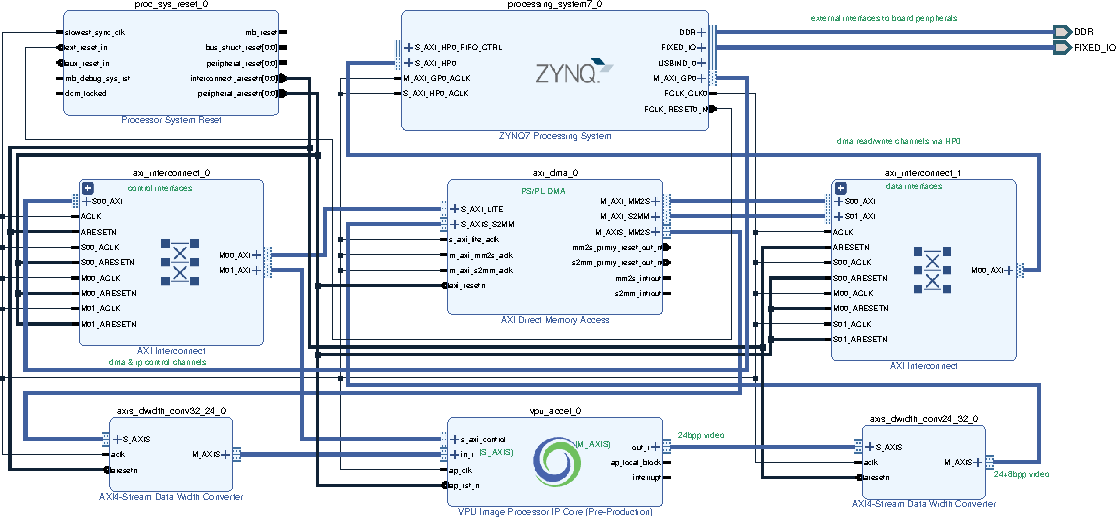
\includegraphics[width=1.2\textwidth]{hw-block-diagram-crop-asset.pdf}}
			\vspace{0.5cm}
			(please see \textit{Appendix}\verwijzingn{paragraaf}{Integrated Block Design Diagram}for a magnified version)

		\end{figuur}

		I've made the decision to only use one global clock net which connects to all components, because I want to prevent components from running off-sync and causing data integrity problems.
		This clock net is derived from the 100MHz system clock.
		As for the reset signal, I had to create different signals for the interconnects and peripherals because those systems cannot be reset at the same time.
		I used the Processor System Reset component to create these reset signals and I connected the interconnect to the reset ports of the interconnects and data width converters.
		The DMA interface and our Image Processor are connected to the peripheral reset net because these need to be reset after the interconnects are up.

		\bigskip

		The Zynq Processing System has multiple types of AXI interfaces, including General Purpose (GP) interfaces and High Performance (HP) interfaces.
		Although it would be easy to put every component on the HP interface, this is not the proper way to do it.
		For good measure, I have connected the control interfaces of the DMA and the Image Processor to the GP interface using an interconnect.
		Only the DMA interfaces which need to be low-latency are connected to the HP interface.
		This is done using a dedicated interconnect.

		\textbf{[todo:]}

	\end{hoofdstuk}

	\begin{hoofdstuk}{Hardware Layer}

		\begin{paragraaf}{Memory Layout}

			The problem I faced regarding the storage of the video frames had to do with the limited amount of Block RAM (BRAM) on the FPGA.
			The camera outputs an image of 640 by 480 pixels with a configurable color channel configuration of RGB444, RGB555 or RGB565.
			We prefer to have the highest color depth due to the image processing algorithm working better if there is more input variance.
			The Arty A7-35T, our target FPGA board, only has $1,800$ kibibits of BRAM, which is not enough to store a full image frame of the lowest color configuration, as can be seen in \verwijzingb{tabel}{Required space to store images of different sizes}.
			One technique to fit the image into memory is to downscale it, but we would lose information on image features which would have an impact on the quality of detection.

			\begin{tabel}{Required space to store images of different sizes}{l @{\extracolsep{\fill}} r r}
				\emph{Bits per channel (BPC)} & 640$\times$420 px & 320$\times$240 px \tabularnewline
				\midrule
				4+4+4 = 12 b & 3150 Kib & 900 Kib \tabularnewline
				5+5+5 = 15 b & 4500 Kib & 1125 Kib \tabularnewline
				5+6+5 = 16 b & 4800 Kib & 1200 Kib  \tabularnewline
			\end{tabel}
			
			The alternatives places to store an image are the 16 MiB of Quad-SPI flash or the 256 MB DDR3L SDRAM.
			The QSPI flash memory has two downsides: it requires controller logic which is only available as an IP Core with a full AXI4 bus, making it difficult to use, and it is shared with the MicroBlaze flash sector, so we would have to make sure that we don't overwrite those contents.
			The DDR3L SDRAM has one major downside: it requires the use of the proprietary Xilinx Memor Interface Generator (MIG) which Digilent does not provide any support for.
			The MIG provides little to no abstraction over the raw DDR3 protocol, making it a challenge of its own to implement it.
			Besides, it is a soft IP, which means that it is delivered in a generic way and the developer has to tailor it to the specific board.
			What makes the SDRAM appealing is its high input clock speed of 166MHz and the ability to read/write 128 bits of information per cycle.
			This high data throughput would mean that we would not have to worry about speed limitations.
			However, the trade-off between the complexity of implementing the memory interface and the benefits that it would bring would need to be considered.

			\bigskip

			The problems with the memory on the Arty A7 development board as I described above made me question the choice of using this particular board.
			I reevaluated the choice and started exploring other development boards.
			Along the way, I discovered the Zynq-7000 SoC lineup that is officially supported by the Vitis Vision libraries.
			One of the cheapest boards available that has a Zynq-7000 SoC is the TUL PYNQ-Z2.
			The SoC on this development board provides a predefined AXI interconnect between the PL and PS which connects the SDRAM via AXI buses.
			In the PL, this SDRAM can be accessed using a hard IP VDMA controller which provides data over AXI Stream buses.
			These AXI Stream buses can be connected to those on the the Vitis Vision HLS-generated RTL solution.
			Another reason why I chose the PYNQ-Z2 is its larger BRAM capacity; it has 4900 Kib of BRAM.
			However, if using the PYNQ Processing System, this memory will be shared with the processor component, leaving a smaller usable space.
			My final decision is to use the DDR3 SDRAM because it is plentyful on the Z2 board: all 512 MB is available to the developer.

		\end{paragraaf}

		\textbf{[todo:]}

	\end{hoofdstuk}

	\begin{hoofdstuk}{Programmable Logic Layer}

		\begin{paragraaf}{Lane Detection IP}

			% ----- Introductie; wat is HLS en Vitis Vision?
			I chose to implement the image processing stages using High Level Synthesis because Xilinx provides a well-designed OpenCV port that is tested and formally proven.
			This port was formerly called xfOpenCV prior to it being integrated into the Vitis standard libraries and renamed to Vitis Vision.
			It is a clean-room implementation of OpenCV functions that includes instruction pragmas which tell the compiler how certain code should be synthesized to RTL.
			These pragmas include information on how certain loops should be unrolled and how variables can be synthesized to registers.
			The developer can write C++ code which specifies which AXI interfaces have to be created and which vision functions have to be applied.
			This code can be simulated on the developer's system using the official OpenCV library to verify the working of the code.
			Once verified, the code can be synthesized to HDL and can be co-simulated to verify that the automatically generated HDL performs exactly like the original code.
			Finally, Vivado can synthesize the HDL to a netlist and implement it into an IP Core, which can be used in other projects.
			

			\bigskip

			% ----- Hoe heb ik de vision libs gebruikt?
			\textbf{[todo: leg uit, een AXI stream voor input en voor output]}

			\bigskip

			% ----- Hoe heb ik de IP Core geintegreerd in het systeem
			I incorporate this IP Core into the block design using IPI and connect the AXI Streams
			\textbf{[todo:]}

		\end{paragraaf}

		\textbf{[todo:]}

	\end{hoofdstuk}

	\begin{hoofdstuk}{Processing System Layer}

		\textbf{[todo:]}

	\end{hoofdstuk}
	
	\begin{hoofdstuk}{Software Layer}

		\textbf{[todo:]}

	\end{hoofdstuk}
	
	% Bibliography page
	\begin{hoofdstuk}{References}

		\printbibliography[heading=none]

	\end{hoofdstuk}

	%\appendix

	\begin{appendices}
		\begin{hoofdstuk}{Enlarged Figures}
			\begin{paragraaf}{Integrated Block Design Diagram}
				\vspace{0.25cm}
				\centerline{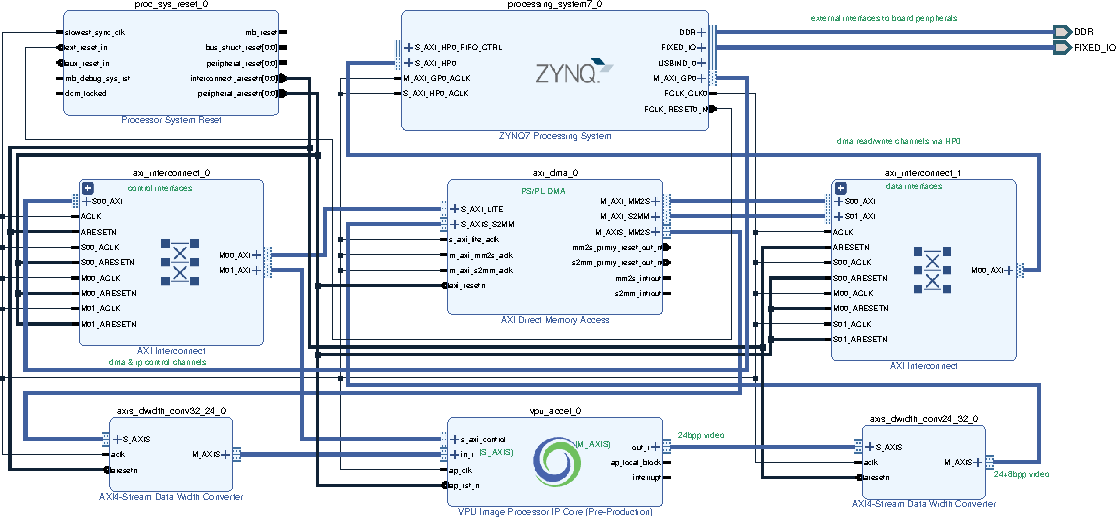
\includegraphics[angle=90, origin=c, clip, trim=9.45cm 0 0 0, width=1.25\textwidth]{hw-block-diagram-crop-asset.pdf}}
				\clearpage
				\centerline{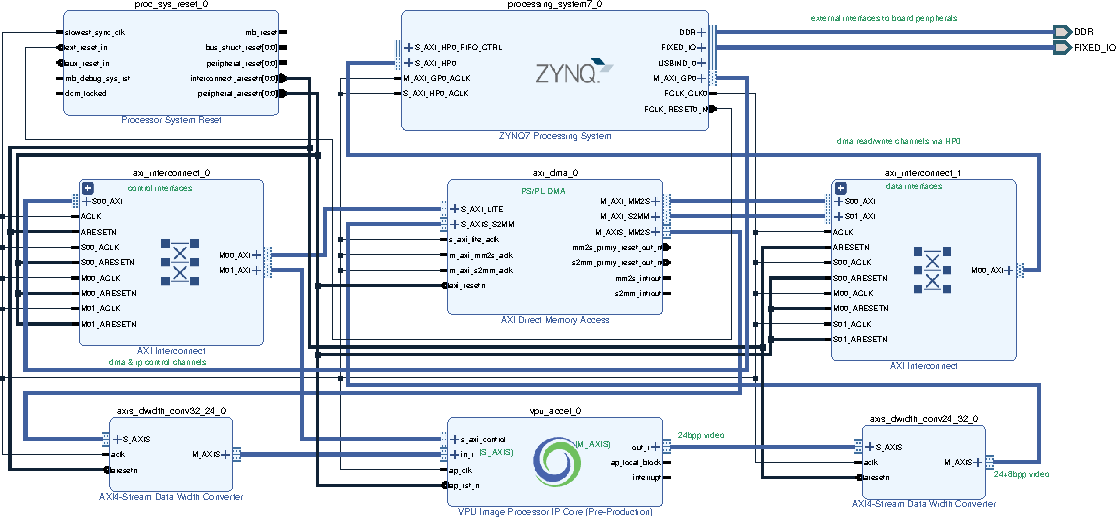
\includegraphics[angle=90, origin=c, clip, trim=0 0 9.45cm 0, width=1.25\textwidth]{hw-block-diagram-crop-asset.pdf}}
			\end{paragraaf}
		\end{hoofdstuk}
	\end{appendices}

	% Empty last page
	\clearpage
	\thispagestyle{empty}
	\addtocounter{page}{-1}
	\ThisULCornerWallPaper{1.005}{asset_bg_last_page.jpg}
	\
	\clearpage

\end{document}
